% UTF-8 encoding
\documentclass[9pt, dvipsnames]{beamer} %
% Beamer 
\usepackage[frenchb]{babel}
\usetheme[secheader]{Boadilla} % Beamer : Boadilla
\usecolortheme{beaver} %  Beamer :beaver

\usefonttheme{professionalfonts} % professional 字体
% Package
\usepackage{times}
\usepackage{amsmath}
\usepackage{verbatim}
\usepackage{anyfontsize}
\usepackage{subcaption}
\usepackage{graphicx} 
\usepackage[export]{adjustbox}
\setbeamertemplate{caption}[numbered]
\newcounter{saveenumi}
\resetcounteronoverlays{saveenumi}
\usepackage[multidot]{grffile} 
\usepackage{tabularx} 
\usepackage{tikz}
\usepackage{bm}
\usepackage[makeroom]{cancel}
%%%%%%%%%%%%%%%%%%%

\newcommand{\nn}{\nonumber \\} % newline sans nombre dans align
\newcommand{\mC}{\mathcal{C}} %pour les fonctions de corrélation
\newcommand{\bx}{{\bf x}} %pour les vecteurs en gras
\newcommand{\by}{{\bf y}} %pour les vecteurs en gras
\newcommand{\bq}{{\bf q}}
\newcommand{\bk}{{\bf k}}
\newcommand{\br}{{\bf r}}
\newcommand{\bv}{{\bf v}}
\DeclareMathOperator{\sgn}{sgn}
% Les > et < se comportent normalement si c'est pour supérieur ou inférieur, sinon se comportent comme \langle
\mathchardef\less=\mathcode`<
\mathchardef\greater=\mathcode`>
\DeclareMathDelimiter{<}{\mathopen}{symbols}{"68}{largesymbols}{"0A}
\DeclareMathDelimiter{>}{\mathclose}{symbols}{"69}{largesymbols}{"0B}


\setbeamertemplate{frametitle}{\bfseries\insertframetitle}


\pgfdeclareimage[height=\paperheight,width=\paperwidth]{bgimage}{loma.jpg}
\usebackgroundtemplate{\tikz\node[opacity=0.1,inner sep=0]{\pgfuseimage{bgimage}};}
%%%%%%%%%%%%%%%%%%%

\date{July 16th, 2020}
\author{Paul Gersberg}
\title{Driving effects on model interfaces}
% Méta-données du PDF
\hypersetup{
    pdfauthor={Paul Gersberg},
    pdfsubject={Manuscrit de thèse de doctorat},
    pdftitle={Confinement and driving effects on continuous and discrete model interfaces},
}

\newcommand{\backupbegin}{
   \newcounter{finalframe}
   \setcounter{finalframe}{\value{framenumber}}
}
\newcommand{\backupend}{
   \setcounter{framenumber}{\value{finalframe}}
}

%%%%%%%%%%%%%%%%%%%%%%%%%%%%%%
%%%%%%%%%%%%%%%%%%%%%%%%%%%%%%
%%%%%%%%%%%%%%%%%%%%%%%%%%%%%%
%%%%%%%%%%%%%%%%%%%%%%%%%%%%%%
%%%%%%%%%%%%%%%%%%%%%%%%%%%%%%

\begin{document}

    \everymath{\displaystyle}

%%%%%%%%%%%%%%% Page de garde
\begin{frame}
    \centering
    
\includegraphics[height=20pt]{anr.png}
    \hfill 
    
\includegraphics[height=20pt]{loma.png}      
    \hfill
    
\includegraphics[height=20pt]{u-bordeaux.png}           
    \hfill
    
\includegraphics[height=30pt]{cnrs.png}
    \hfill
    
\includegraphics[height=20pt]{logo_ENS.jpg}        
    \vfill
    {École doctorale 209 : Sciences physiques et de l'ingénieur}\\
    \vfill
    { THESIS}\\
    {\bfseries \scriptsize to obtain a PhD from}\\
    {\bfseries Université de Bordeaux}\\
    {{\bfseries Spécialité doctorale ``Laser, Matière, Nanosciences``}}\\
    \textit{\scriptsize presented by }\\
    {{\Large \bfseries Paul Gersberg}} \\
    {\scriptsize on July 16th 2020} \\
    \vfill
    {\huge \color[rgb]{0,0,1} \bfseries{Confinement and driving effects on continuous and discrete model interfaces}} \\
    \vfill
    \raggedright
    {\bf PhD director :} David S. Dean, LOMA \\
    {\bf PhD co-director :} Peter C.W. Holdsworth, ENS Lyon \\
    \textbf{\scriptsize Université de Bordeaux, Laboratoire Onde Matière d'Aquitaine, 351 Cours de la Libération, Talence, France}

\end{frame}

\begin{frame}
    \frametitle{Content}
    \tableofcontents
\end{frame}

%%%%%%%%%% Interface definition
\section{Statistical description of physical systems}

\begin{frame}
    \frametitle{Statistical systems}
    Collective behavior from a large number of degrees of freedom \\
    \begin{overprint}
	    \onslide<1>
	    \centering
	    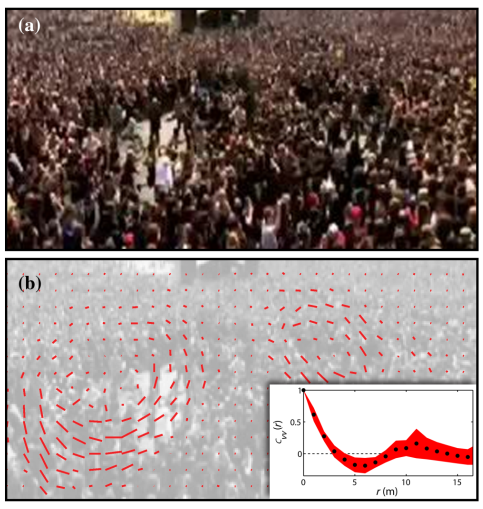
\includegraphics[scale=0.3]{mosh-pit.png} \\
	    {\it Collective Motion of Humans in Mosh and Circle Pits at Heavy Metal Concerts [Silverberg et al. 2013]} \\[0.5cm]
	    Order parameter: mean people's density (conserved)
	    
	    \onslide<2>
	    \centering
	   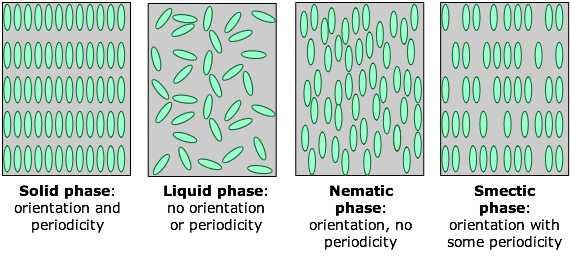
\includegraphics[width=\linewidth]{nematic-smectic.jpg} \\
	   {\it Schematics of liquid crystals [Chem.libretext.org] }\\[1cm]
	   Order parameter : mean liquid crystal's orientation (non-conserved)
   \end{overprint}
\end{frame}
%
%\subsection{Ising model}
%\begin{frame}
%    \frametitle{Ising model}
%    Discrete lattice model, each site has value $\sigma_i = \pm1$ \\
%    \centering
%    
\includegraphics[scale=0.7]{ising.pdf} \\
%    {\it 2D Monte Carlo simulation at $T=0.8T_C$ } during coarsening\\[1cm]
%    Order parameter : mean magnetization $M = \frac{1}{N} \sum_i \sigma_i$ \\
%    Conserved (canonical) or non-conserved (grand-canonical) \\
%    Mapping to liquid/gaz, gaz adsorption, binary fluids
%\end{frame}


\begin{frame}
    \frametitle{Statistical field theory}
    Continuous field $\phi(\bx,t)$  : density, magnetization, orientation... {\footnotesize [Hohenberg et Halperin 1977 (18),Bray 1994 (22)]} \\
    Total order parameter : $\Phi(t) = \int d\bx \phi(\bx,t)$ 
    \begin{block}{Brownian field dynamics}
		\begin{align}
    		\frac{\partial \phi(\bx)}{\partial t} = - L \frac{\delta H}{\delta \phi(\bx)} + \eta(\bx,t)  &~,~  < \eta(\bx,t)\eta(\bx',t)> =\delta(t-t')\Gamma(\bx,{\bf x'}) \\
           p(\phi) = \exp(-\beta H[\phi]) &~, ~	\Gamma(\bx,\bx') =2T L(\bx,\bx')
		\end{align}    
    \end{block}
    \begin{columns}
    \column{0.45\linewidth}
    \begin{block}{Grand Canonical ensemble : \\ {\bf model A}} 
         $\Phi(t) \neq cte$ \\
        $L(\bx,\bx')=\textcolor{blue}{\alpha}\delta(\bx-\bx')$,
		\begin{equation}
    		\frac{\partial \phi(\bx)}{\partial t}= -\textcolor{blue}{\alpha} \frac{\delta H}{\delta \phi(\bx)} + \eta(\bx,t) 
		\end{equation}
		Discrete : {\bf Glauber} dynamics
    \end{block}    

    \column{0.45\linewidth}
%    \vspace{-0.45cm}
    \begin{block}{Canonical ensemble : \\ {\bf model B}}
        $\Phi(t) = cte$ \\
        $L(\bx-\bx')= -\textcolor{blue}{D\nabla^2} \delta(\bx-{\bf x'})$
		\begin{equation}
    		\frac{\partial \phi(\bx)}{\partial t}= \textcolor{blue}{\nabla}\cdot[ \textcolor{blue}{D\nabla } \frac{\delta H}{\delta \phi(\bx)} + {\boldsymbol\eta}(\bx,t)]
		\end{equation}
		Discrete : {\bf Kawasaki} dynamics		
    \end{block}
    \end{columns}
\end{frame}


\section{Interface definition}

\begin{frame}
    \frametitle{Phase separation}
        \begin{block}{Ginzburg-Landau Hamiltonian [Landau et Lifschitz 1990 (1)]} 
        \begin{align}
            H[\phi] = \int d\bx  \underbrace{\frac{\kappa}{2}[\nabla \phi]^2}_{\text{cost of changing $\phi$}} + \underbrace{V(\phi)}_{\text{phase separating potential}}
        \end{align}
       	\end{block}

       	\begin{block}{$\phi^4$ potential}
			\begin{columns}
			\column{0.4\linewidth}
			\begin{overprint}
			\onslide<1>
       		\begin{align}
       			V(\phi) = \frac{1}{2} (T-T_C) \phi^2 + \frac{\lambda}{4!} \phi^4
       		\end{align}
       		\onslide<2>
       		\begin{align}
       			V(\phi) = \frac{1}{2} (T-T_C) \phi^2 &+ \frac{\lambda}{4!} \phi^4 \nn 
       			&{\color{gray} \bf + B \phi}
       		\end{align}       		
       		\end{overprint}
       		
			\column{0.52\linewidth}       		
       	\centering
        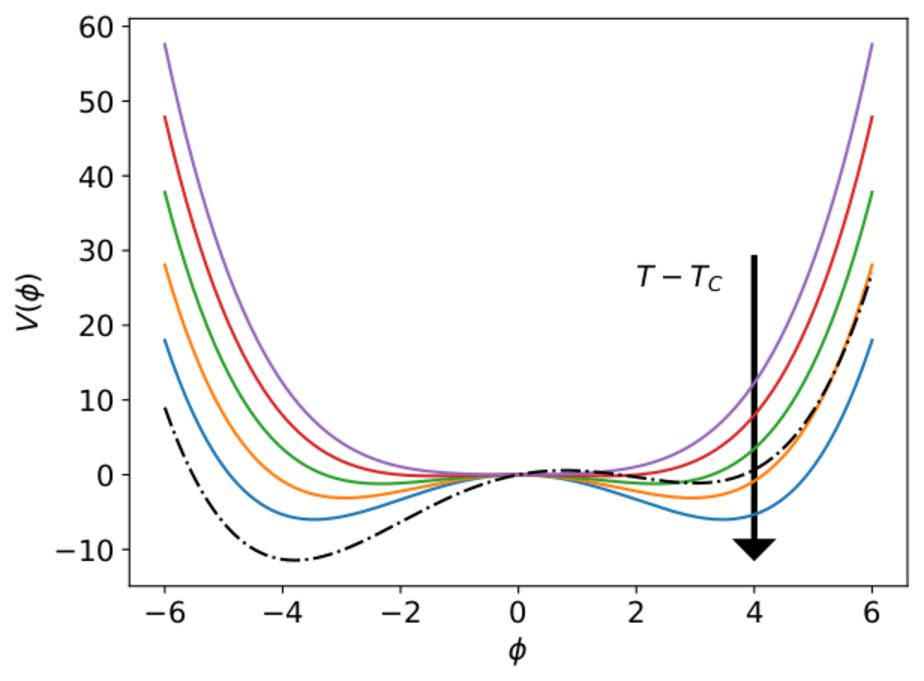
\includegraphics[width=\linewidth]{double-puit-en-fonction-temp.pdf}
        \end{columns}
       	\end{block}        
\end{frame}

\begin{frame}
	\frametitle{Interface between two coexisting phases}
	\begin{block}{Mean-field equilibrium system (dynamic independent)}
		\begin{align}
			\cancel{\frac{\partial \phi(\bx)}{\partial t}} = - L \frac{\delta H}{\delta \phi(\bx)} + \cancel{\eta(\bx,t)}  \implies  \frac{\delta H}{\delta \phi(\bx)} = 0 
		\end{align}
	\end{block}
	\begin{columns}
    \column{0.45\linewidth}	
    \begin{block}{$\phi^4$ mean-field kink solution ($h=0$)}
        \begin{align}
            \phi_K(z) = \tanh \left( \frac{z}{\xi_\perp} \right)
        \end{align}
    \end{block}	
	\begin{block}{Interface SFT approximation}
        \begin{align}
            \phi(\bx,t) &= f(z-h(\br,t)) \\
            \phi_K(z) &= f(z) 
        \end{align}
    \end{block}
    \column{0.45\linewidth}	
    	\centering
		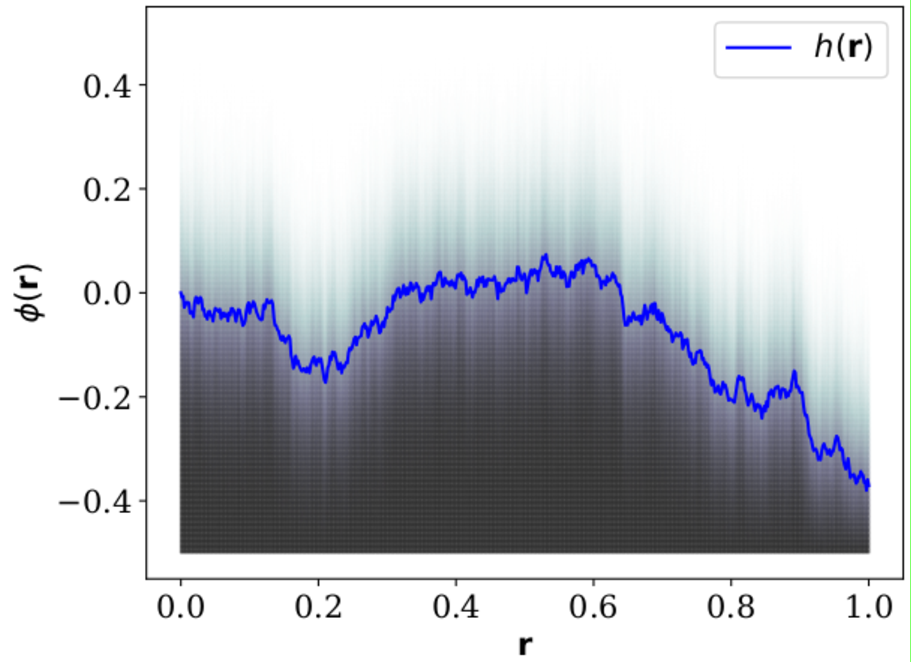
\includegraphics[width=\linewidth]{interface-profil.pdf}
		Interface schematics
	\end{columns}    
\end{frame}

\begin{frame}
    \frametitle{Interface examples}
    \begin{overprint}
        \onslide<1>
            Equilibrium (boundary conditions), grand-canonical (discrete model A - Glauber) \\
	        \centering       
		    
\includegraphics[scale=0.7]{t-85.pdf} \\
		    2D Ising Monte Carlo simulation, $T=0.85 T_C$
        \onslide<2>
            Out-of-equilibrium (initial conditions) surface growth, grand-canonical (model A) \\
	        \centering       
		    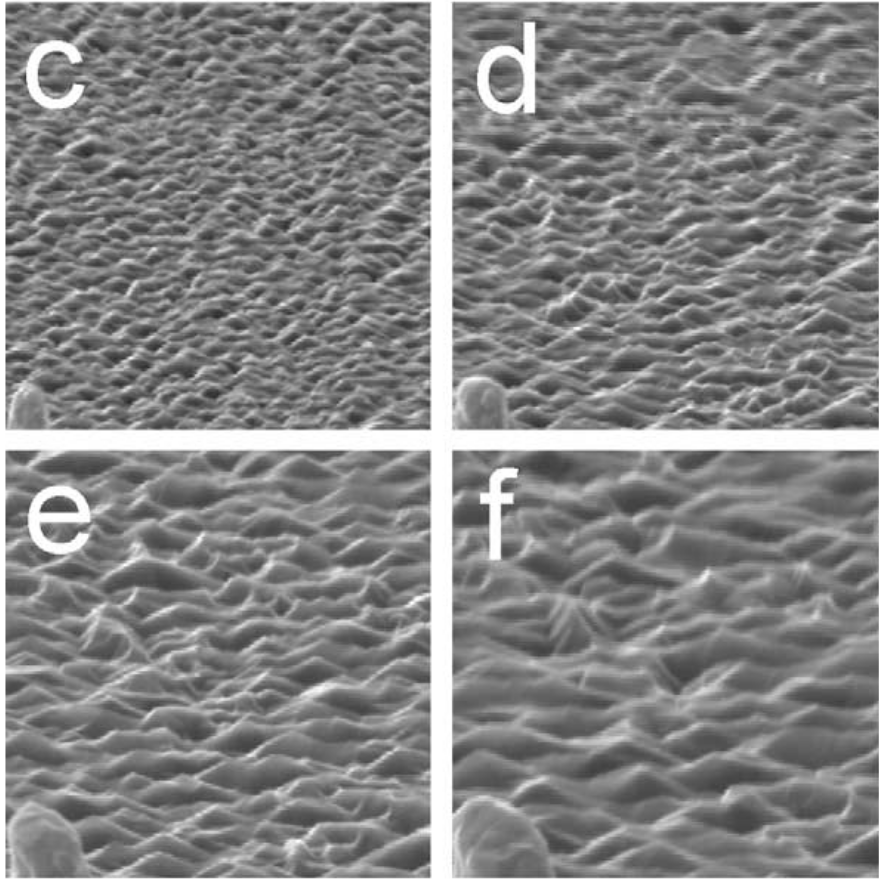
\includegraphics[scale=0.2]{crystal-growth.png} \\
		    SEM movie showing a gallium arsenide film grown on silicon [Finnie et al. 2000]
	    \onslide<4>
	        Out-of-equilibrium (initial conditions), canonical (model B) \\
	        \centering
		    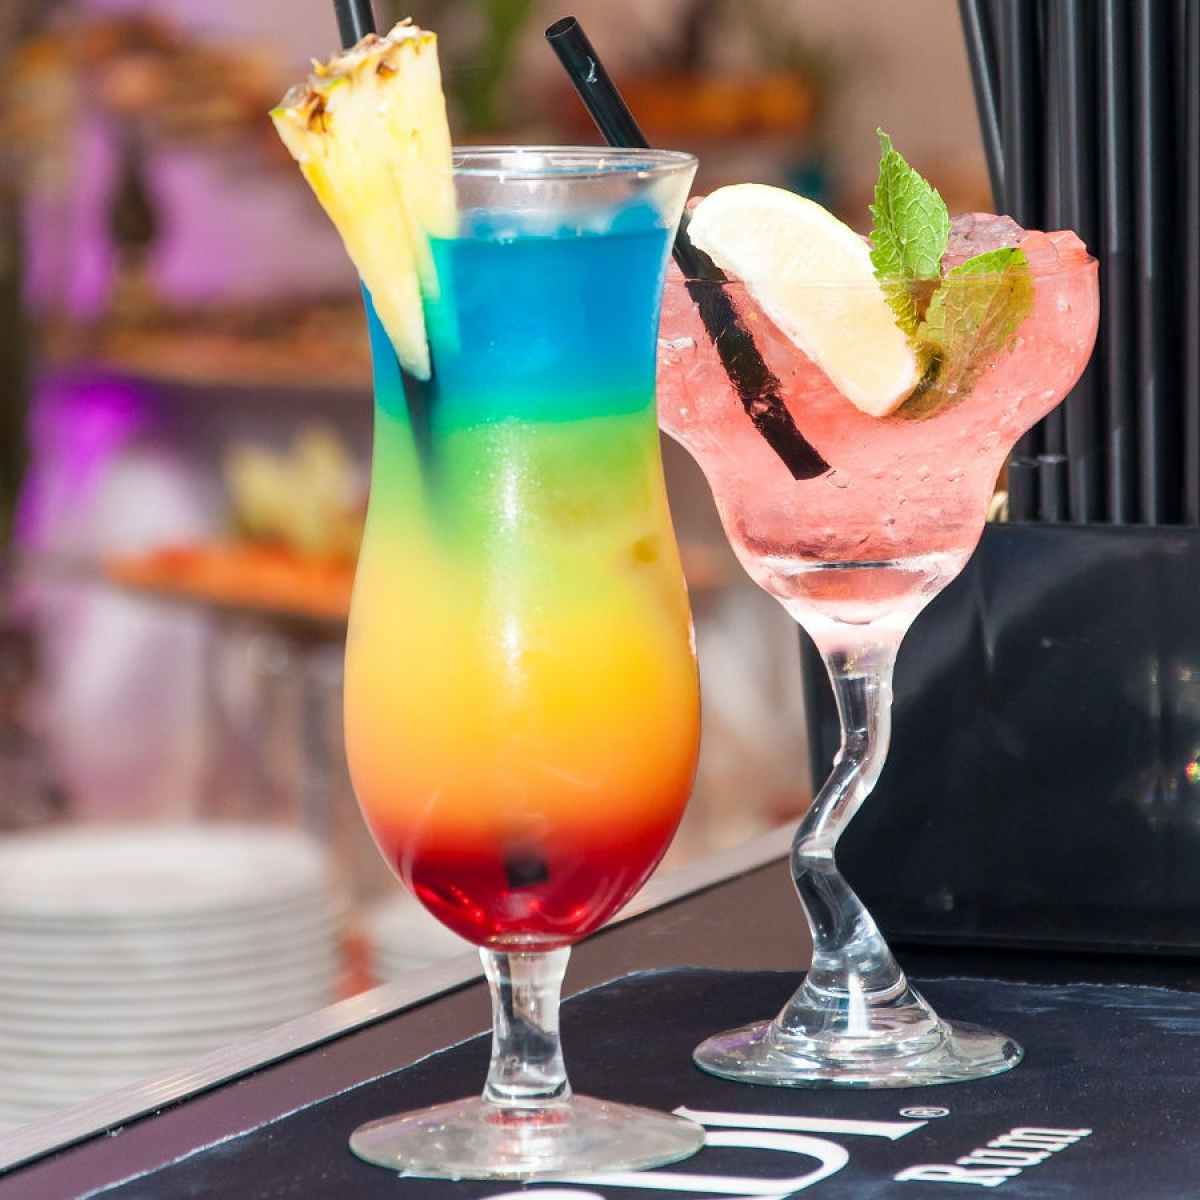
\includegraphics[scale=0.15]{binary-fluid.jpeg} \\
		    Pigment concentration in cocktails [Cocktailmag.fr] 	    
        \onslide<3>
            Equilibrium, canonical (model B) \\
            \centering
            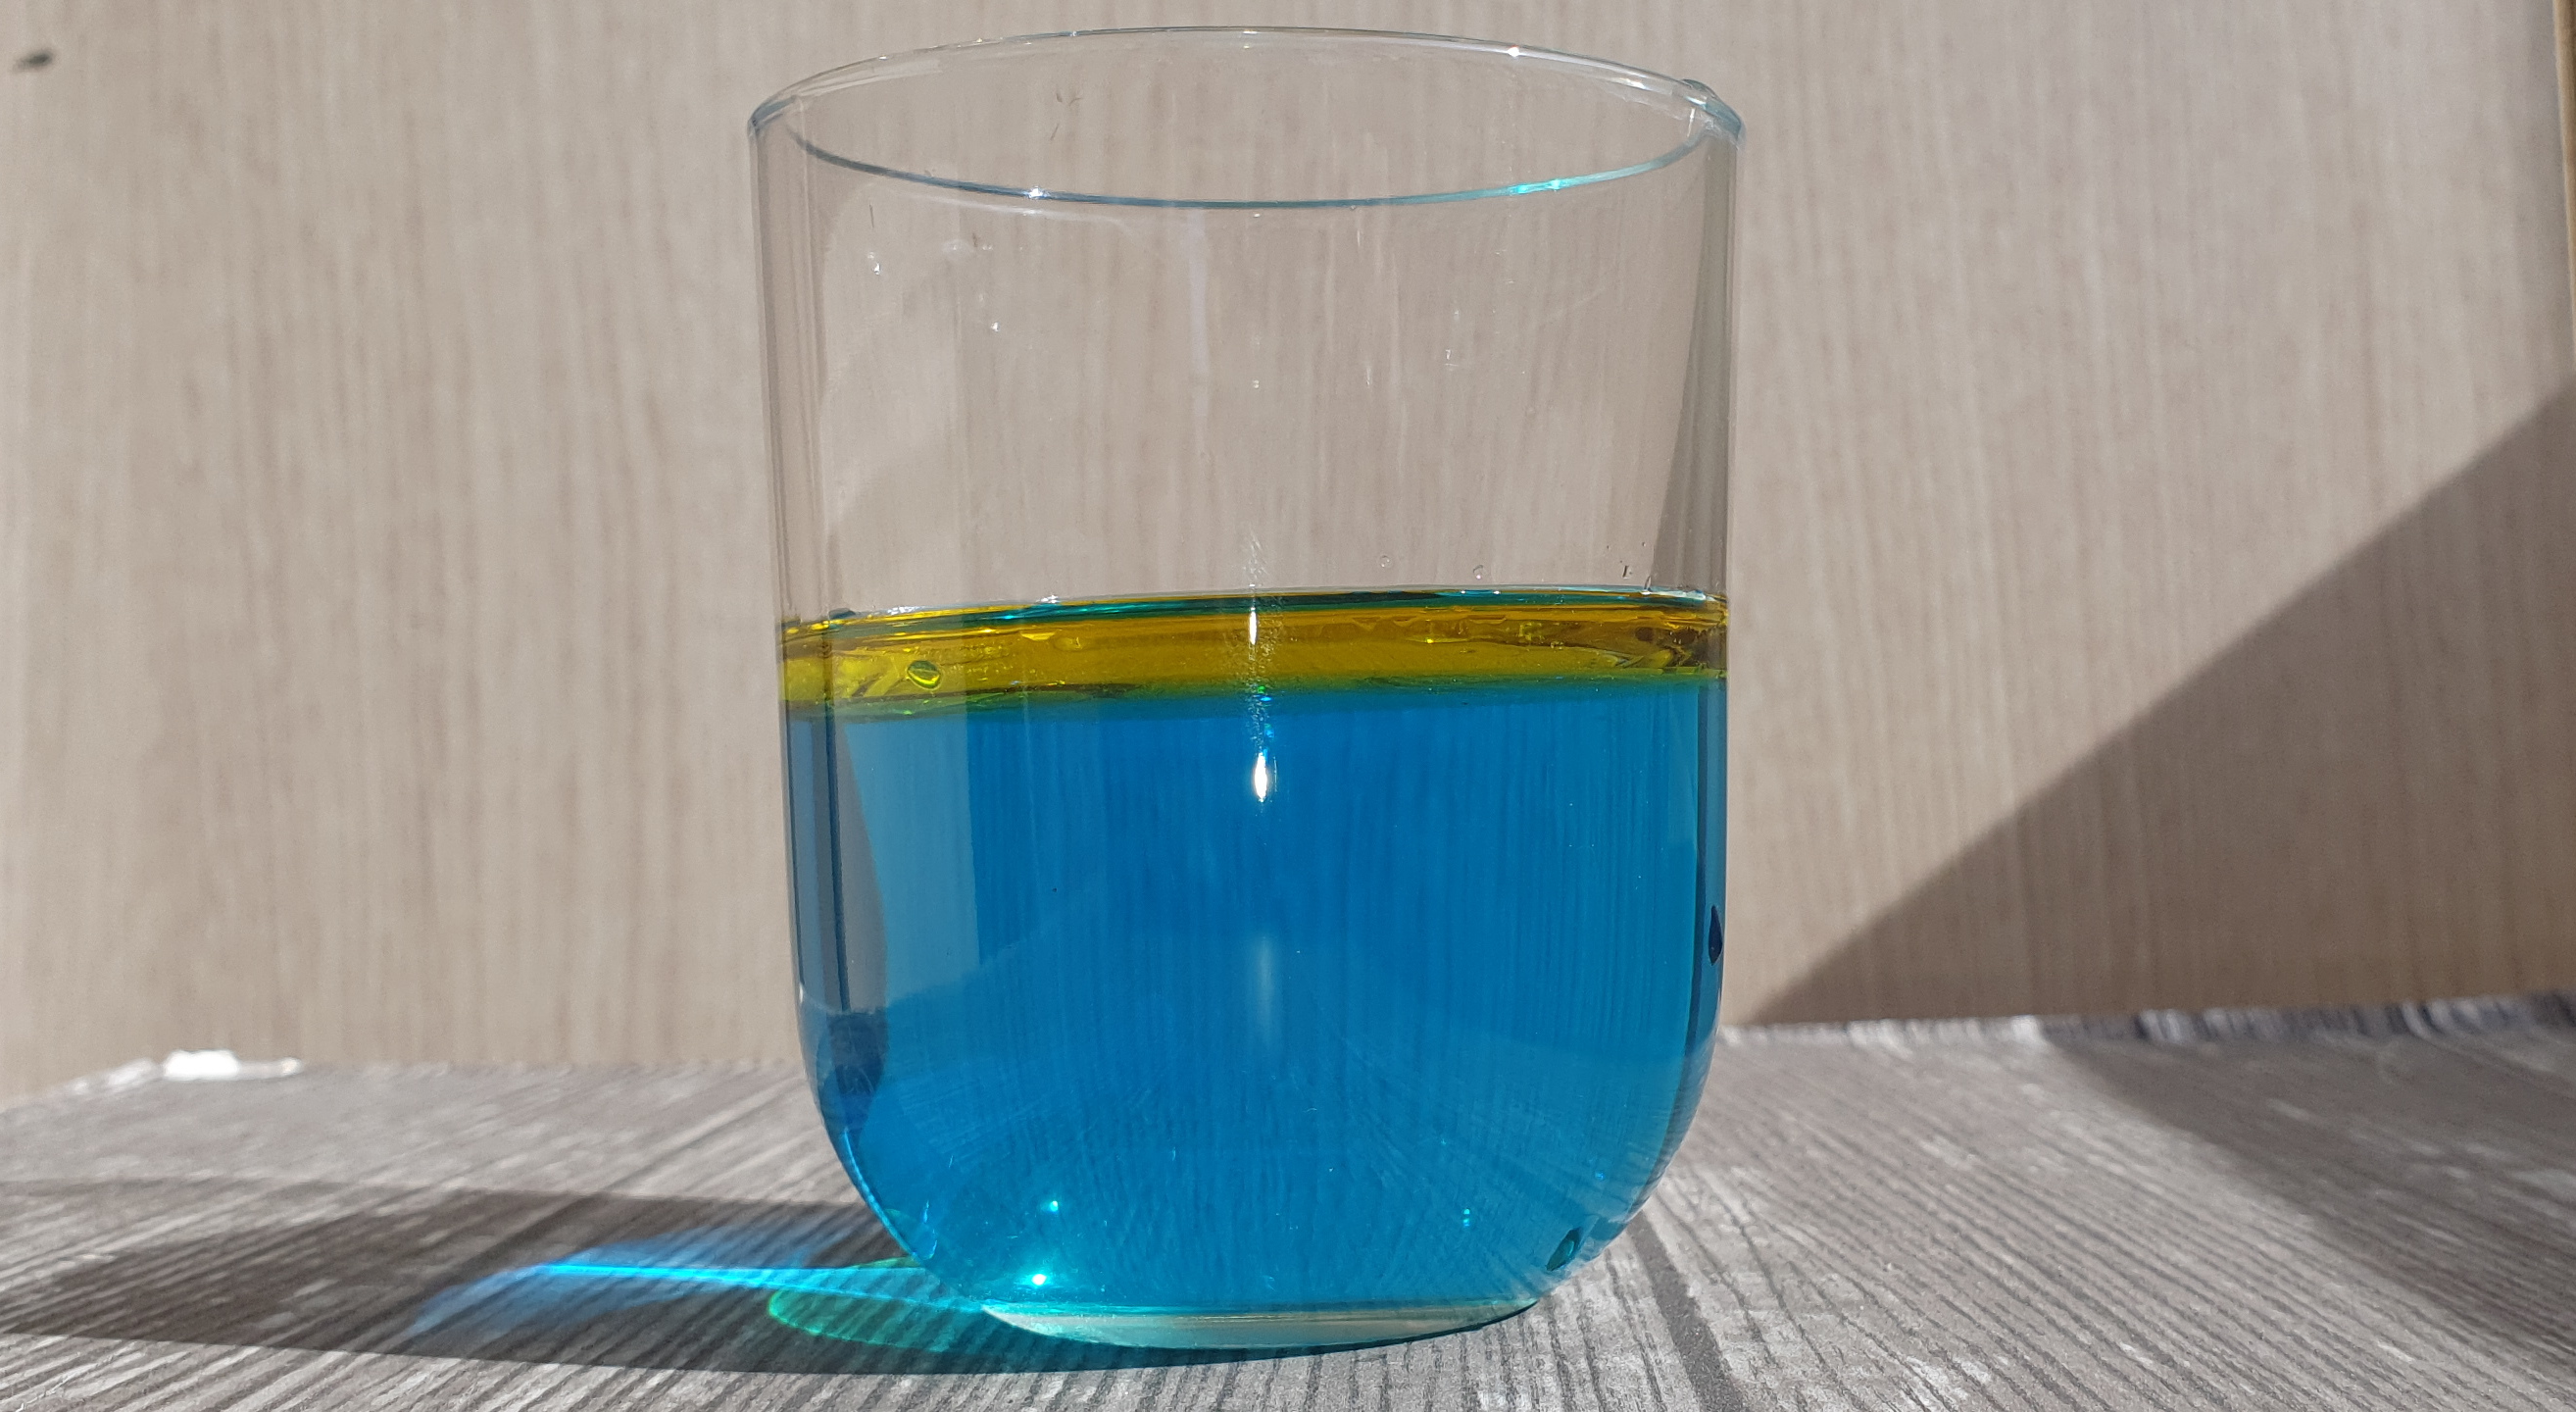
\includegraphics[scale=0.1]{eau-huile.jpg} \\
            Water-oil interface 
	\end{overprint}
\end{frame}

\begin{frame}
    \frametitle{Surface tension}
    \begin{block}{Definition by the free energy [Abrahams et Reed 76 (46)]}
        \begin{align}
            \sigma = f_{interface} - f_{homogeneous}  [E \cdot L^{-2}]
        \end{align}
    \end{block}
    \begin{columns}
    \column{0.45\linewidth}
    \begin{block}{Cahn-Hilliard estimate \newline [Cahn et Hilliard 58 (25)]}
        \begin{equation}
            \sigma= \int dz\ {\kappa}\left(\frac{d\phi_K(z)}{dz}\right)^2 
        \end{equation}    
    \end{block}
    \begin{block}{Limits}
    	\begin{itemize}
			\item $\xi_\perp \to 0$ : sharp interface
			\item $\xi_\perp \to \infty$ : ultra-low surface tension, critical systems 	
    	\end{itemize}
    \end{block}
    \column{0.45\linewidth}
    \begin{block}{    Surface tension with respect to interface width $\xi_\perp$}
    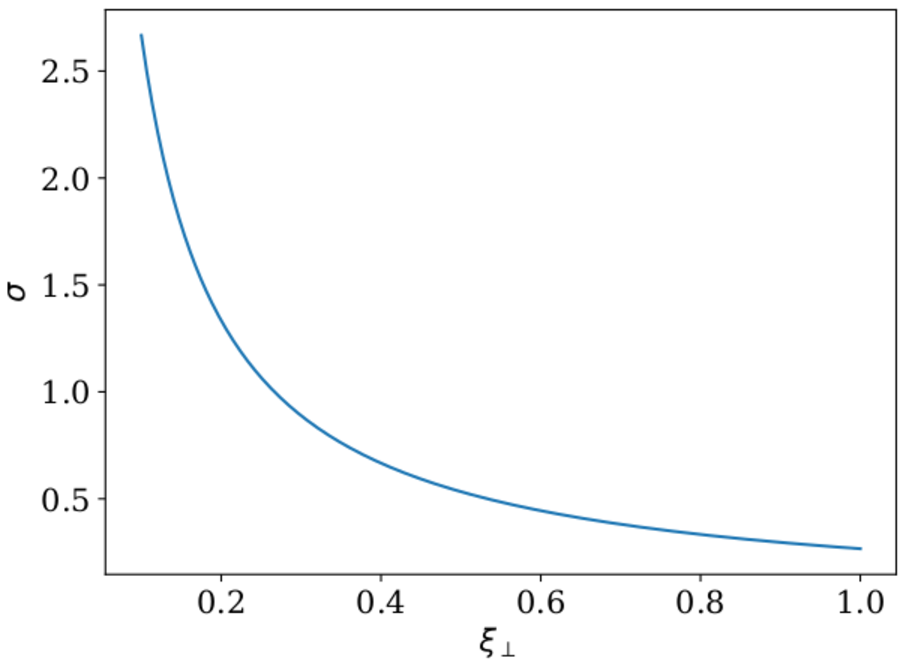
\includegraphics[width=\linewidth]{tension-superficielle.pdf} \\    
    \end{block}
    \end{columns}
\end{frame}

\section{Confinement forces}

\begin{frame}
    \frametitle{Confinement forces [chapter 3]}
    \begin{block}{Excess free energy and Casimir force [Gambassi 09 (3)]}
    \begin{columns}
    \column{0.45\linewidth}
		\begin{align}
		F(t,h,L) = L'^2 \left( L f_{bulk} + \beta^{-1} f_{ex} \right)
		\end{align}
    \column{0.45\linewidth}    
		\begin{align}
		 f_{casimir} = - \beta^{-1} \frac{\partial  f_{ex}}{\partial L}
		\end{align}
    \end{columns}
    \end{block}
    \begin{block}{1D Confined elastic line  $0 \less h(\br,t) \less L$}
	\begin{columns}
	\column{0.45\linewidth}
	    \begin{align}
		   f = \frac{T^2\pi^2}{2\sigma L^2} 
	    \end{align}
	    Finite-size effects surface tension [Privman 1988 (16)] 
	    \begin{align}
	    	\sigma(L) \simeq \sigma_{bulk}+\frac{Ta}{L}
    	\end{align}
	    \begin{align}
	        f_c= \frac{T\pi^2}{2 a L} 
	    \end{align}
	    \column{0.45\linewidth}
	    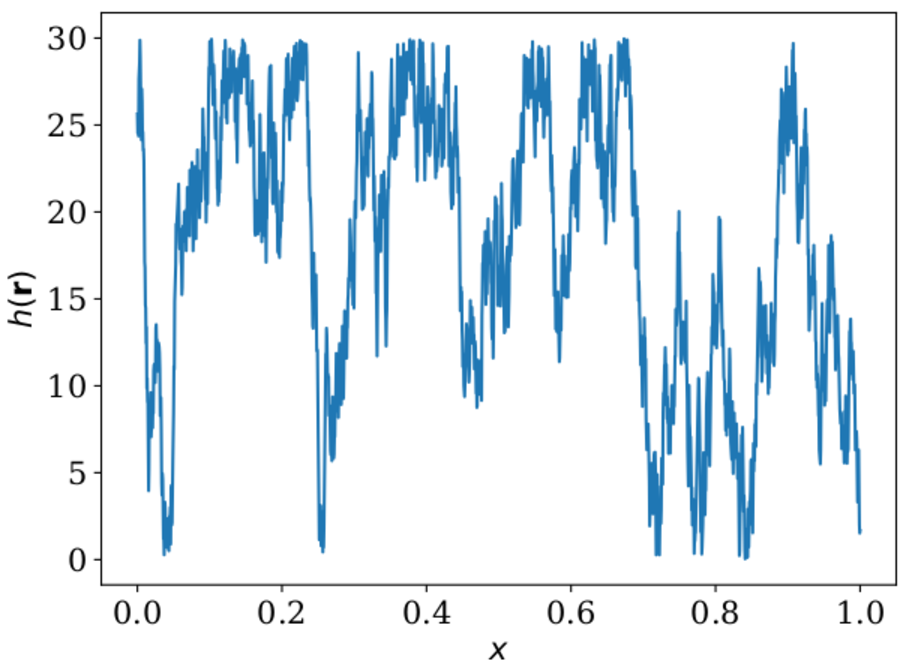
\includegraphics[width=\linewidth]{interface-confined.pdf}
	    {\footnotesize Confined interface for $L_Y=30$ schematics}
	    \end{columns}
	\end{block}
\end{frame}

\section{Out-of-equilibrium steady-states}

\begin{frame}
	\centering
	\huge How do out-of-equilibrium steady-states affect interfaces ?
\end{frame}

\begin{frame}
    \frametitle{Driving at the interface}
    \centering
    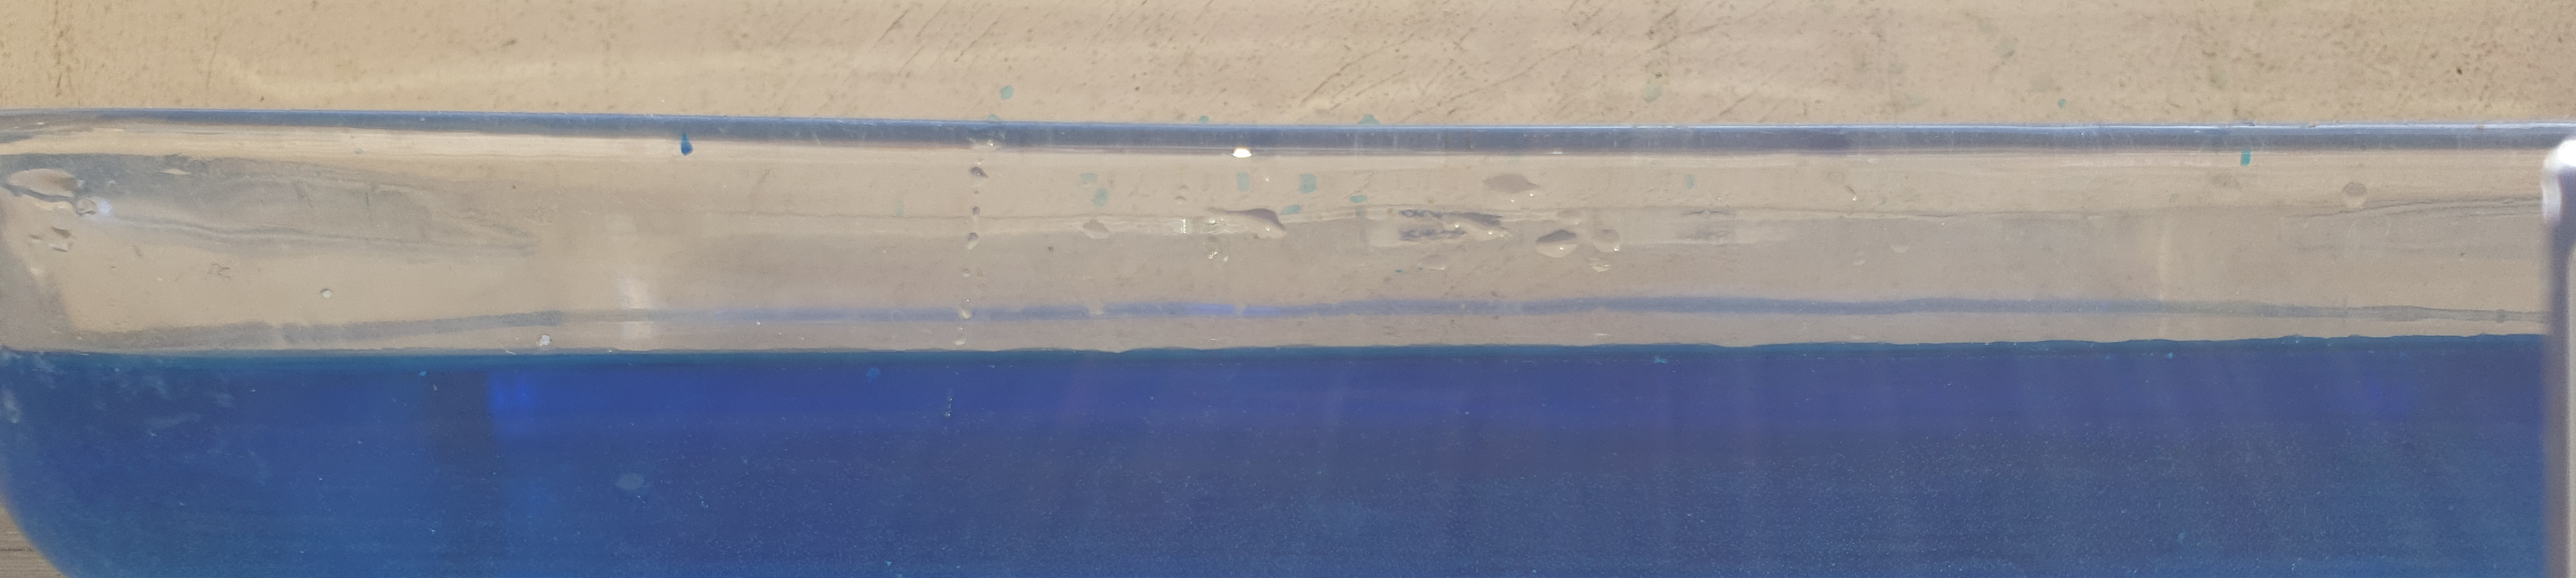
\includegraphics[width=0.8\linewidth]{wave-0.jpg}  \\
    \vspace{0.5cm}
    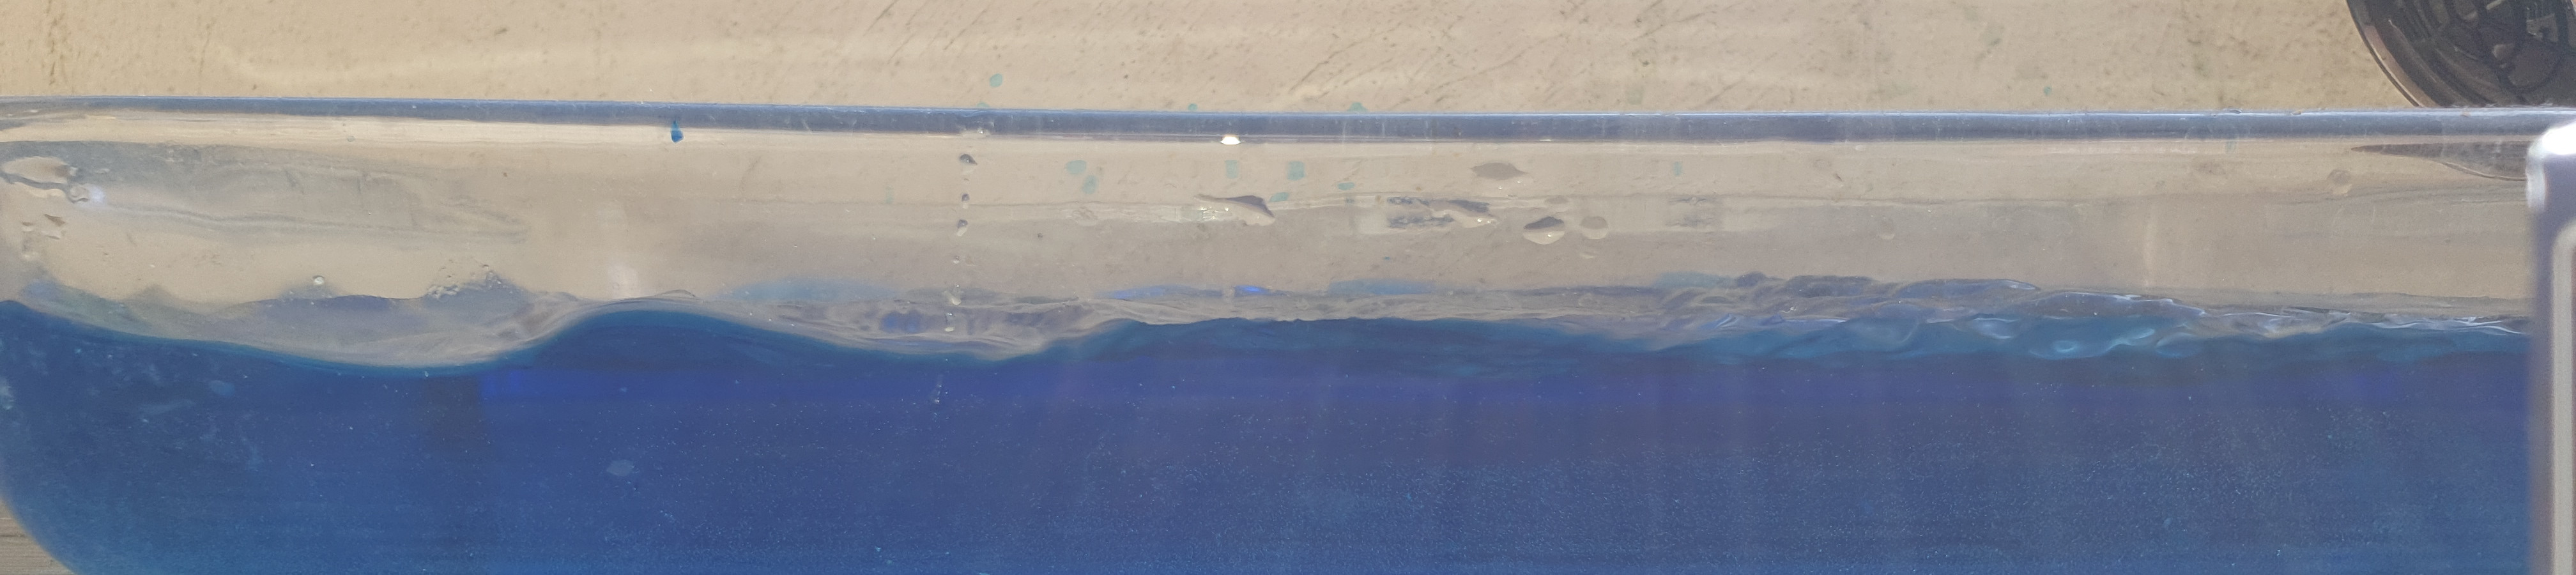
\includegraphics[width=0.8\linewidth]{wave-1.jpg} \\
    \vspace{0.5cm}    
    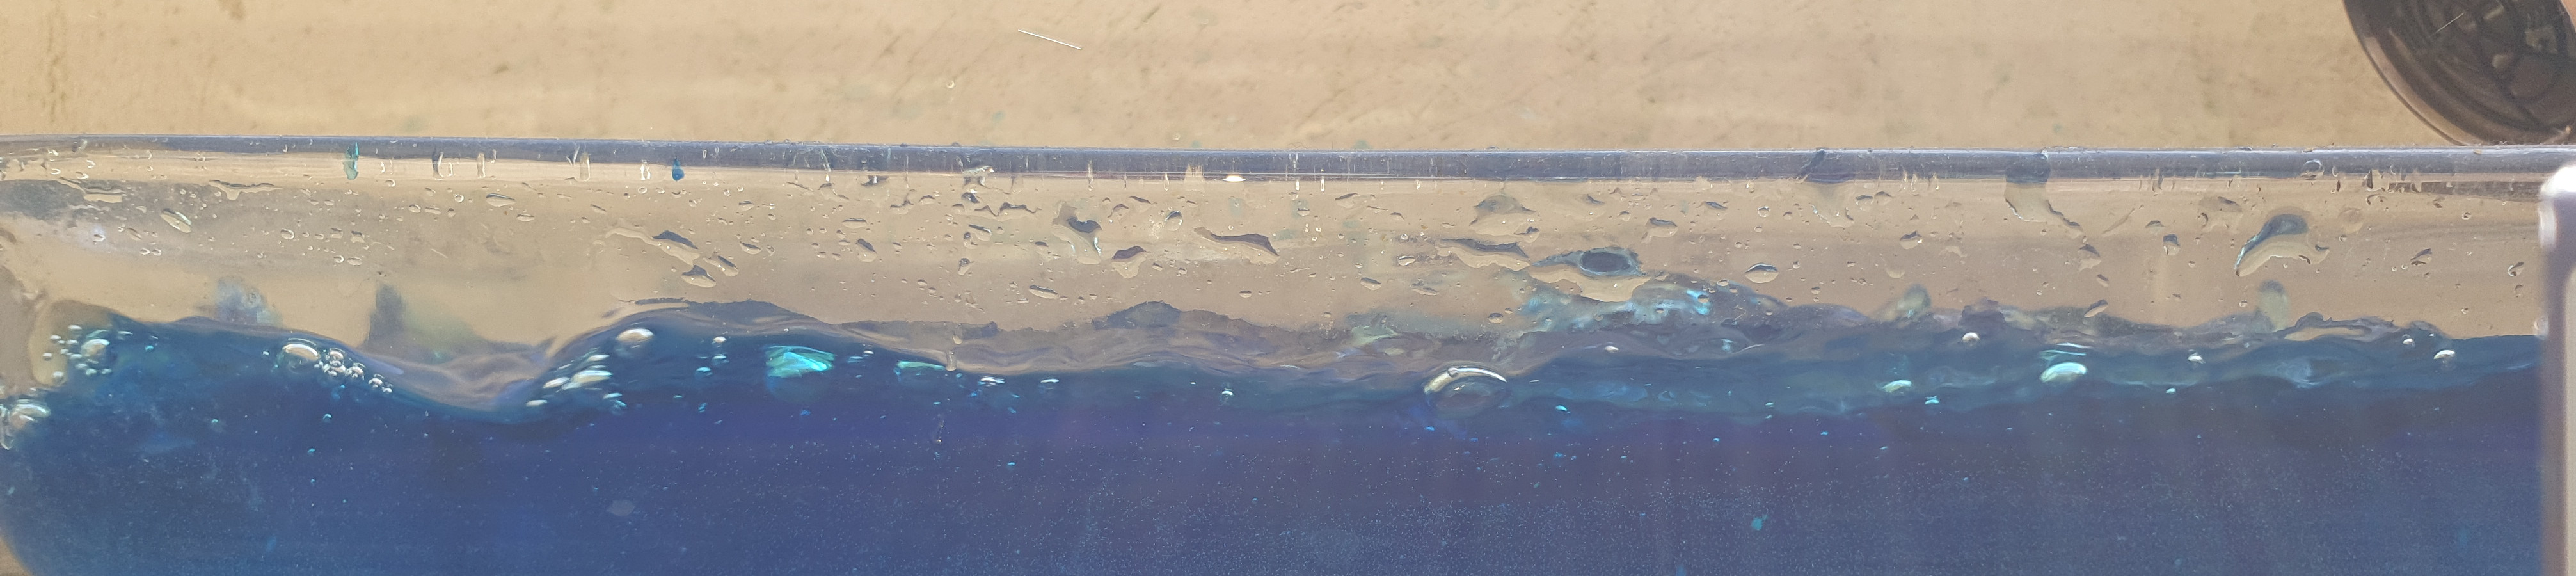
\includegraphics[width=0.8\linewidth]{wave-2.jpg} \\ 
	Home-made wind generated waves (from a hair dryer)
\end{frame}

\begin{frame}
    \frametitle{The Solid-On-Solid model}
    \begin{block}{Solid-On-Solid model}
    	Lattice model with interface height $h_i$
    	\begin{align}
	    	H = J \sum_{i=0}^{L'} |h_i-h_{i+1}| + \mu \sum_{i=0}^{L'} \frac{h_i+h_{i+1}}{2}
    	\end{align}
    \end{block}
    \begin{columns}
    \column{0.45\linewidth}
	\begin{block}{Metropolis algorithm}
		\begin{itemize}
			\item Glauber 
			\begin{align}
				\{h_i\} \to  \{h_i \pm 1\} 
			\end{align}
			\item Kawasaki ($\sum h_i = cte$)
			\begin{align}
				\{h_i,h_{i\pm 1} \} \to \{h_i-1,h_{i \pm 1}+1\} 
			\end{align}			
			\item New configuration with probability 
			\begin{align}A(C\to C') = \exp(-\beta \Delta H)
			\end{align}
		\end{itemize}
	\end{block}
    \column{0.55\linewidth}
    \centering
	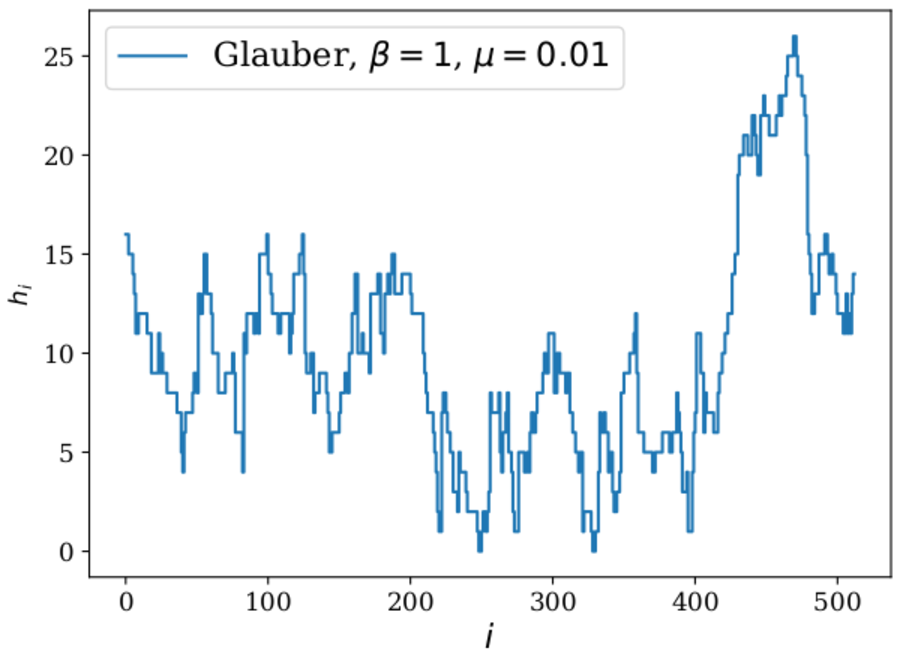
\includegraphics[scale=0.4]{snap-sos.pdf}
    \end{columns}
\end{frame}

\begin{frame}
	\frametitle{Driving at the interface}
		Driving : $\Delta E_{d} = \Delta E_{eq} \pm v$ in Kawasaki dynamics \\
		\begin{overprint}
		\onslide<1>
		\begin{figure}
			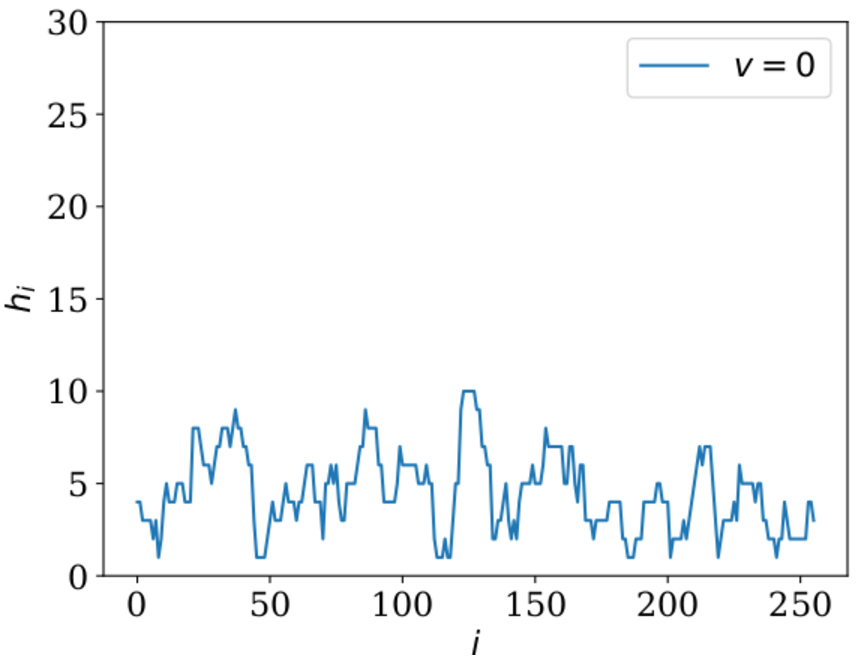
\includegraphics[width=0.35\linewidth]{sos-driving-snaps0.pdf}		
			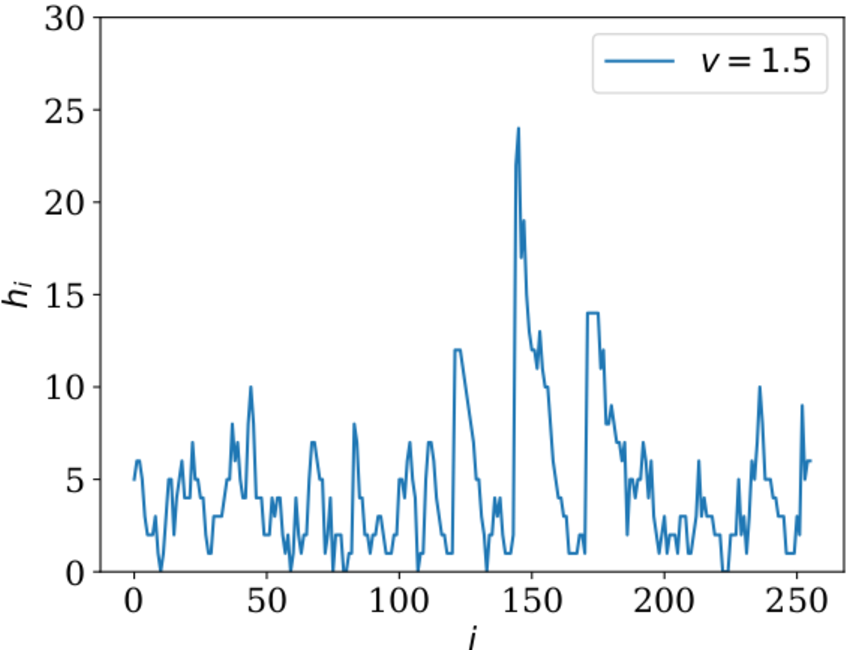
\includegraphics[width=0.35\linewidth]{sos-driving-snaps1.pdf}		
			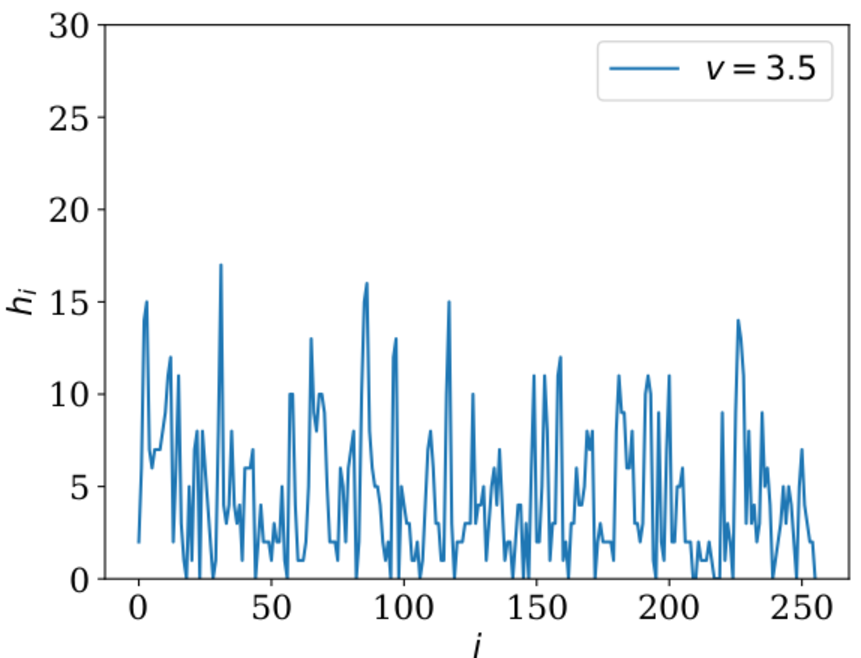
\includegraphics[width=0.35\linewidth]{sos-driving-snaps3.pdf}		
			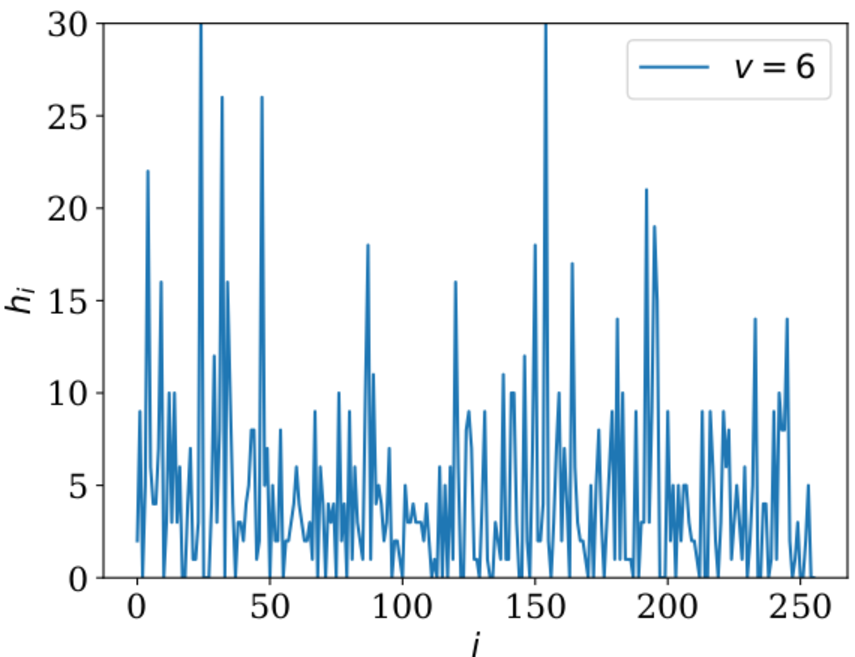
\includegraphics[width=0.35\linewidth]{sos-driving-snaps6.pdf}										\end{figure}				
			\centering
			$\beta = 1, L_Y = 200, \frac{1}{L'}\sum h_i = 4.51$
		\onslide<2>
		\centering
	    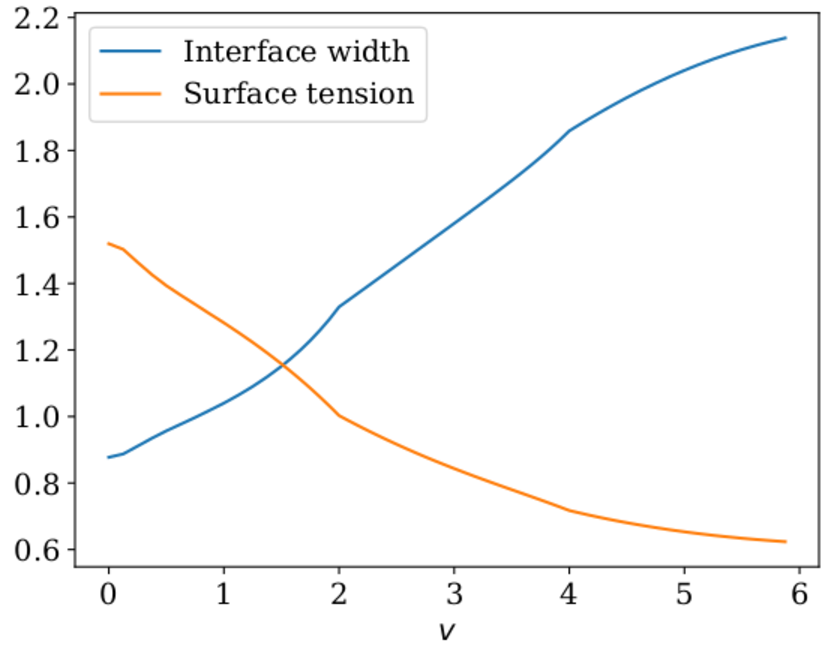
\includegraphics[scale=0.6]{tension-drive.pdf} \\
	    {\small Monte Carlo driving of SOS interface at $\beta=1$ and $\frac{1}{L'}\sum h_i = 4.51$ }
	    \end{overprint}
\end{frame}


\begin{frame}
	\centering
	\huge What happens if we shear not only the interface, but the whole system ?
\end{frame}

\begin{frame}
    \frametitle{PMMA polymers in polystyrene solvent under shear \newline [Derks et al. 2006]}
    \begin{overprint}
    \onslide<1> 
	    \begin{columns}
	    \column{0.3\linewidth}
	    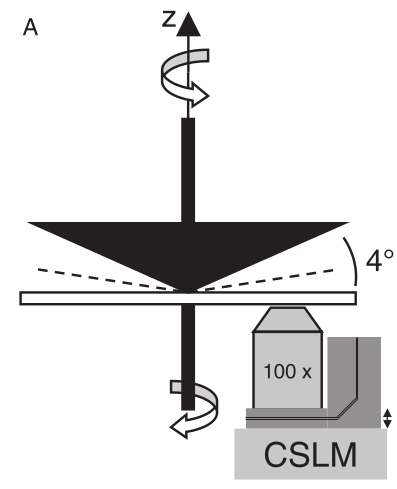
\includegraphics[width=\linewidth]{derks-setups.png}
	    Experimental setup [Derks et al. 2004]
	    \column{0.45\linewidth}
	    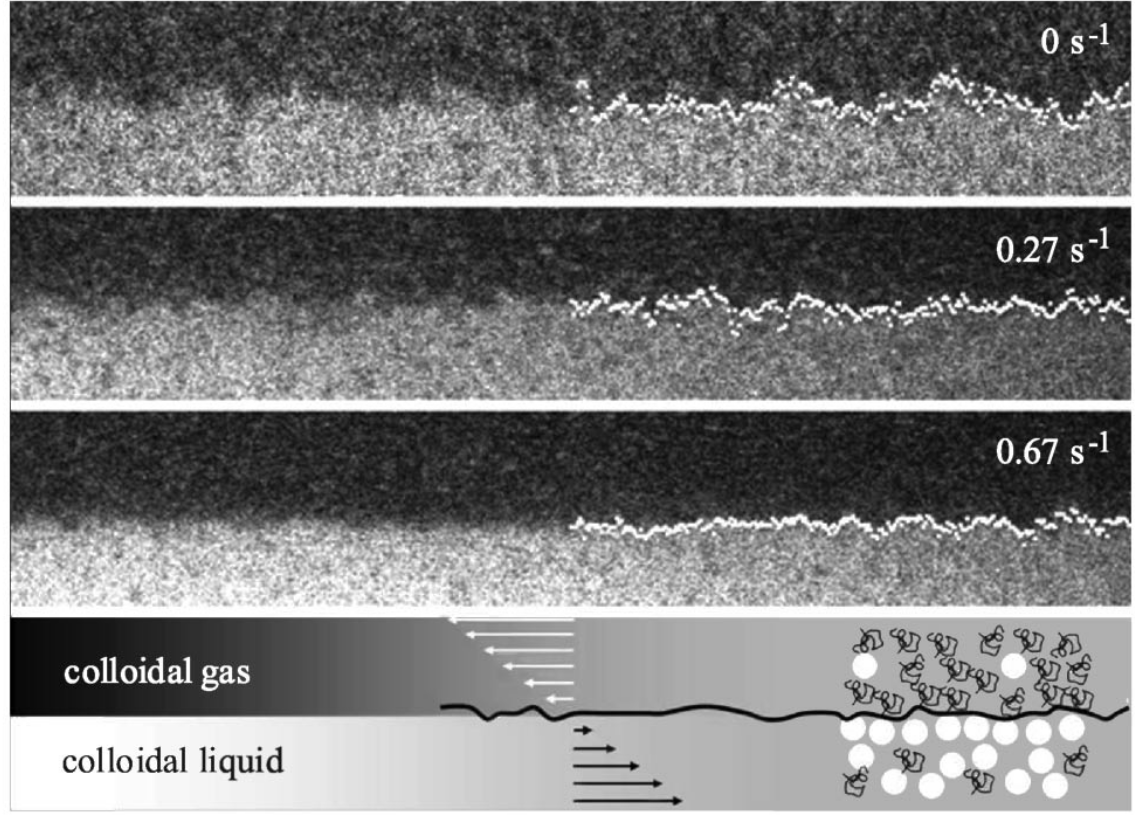
\includegraphics[width=\linewidth]{derks.png} 
	    Interface snapshots under shear [Derks at al. 2006]
	    \end{columns}
	\onslide<2>
	    \begin{columns}
	    \column{0.5\linewidth}
	    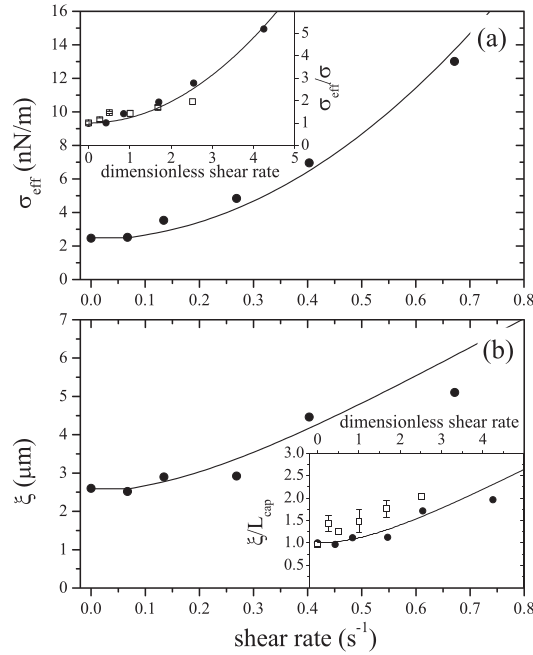
\includegraphics[width=0.9\linewidth]{derks-results.png}
	    \centering
		{\footnotesize  Effective interfacial tension and correlation length \\ along the interface}
	    \column{0.4\linewidth}
	    \begin{block}{Phenomenolocial model}
	    Modes slower than shear rate  no longer contribute to the entropy of the interface
			\begin{align}
			&\sigma_{eff}(\dot{\gamma}) = \nn
			&\sigma + \frac{3 k_B T}{4 \pi} \frac{\dot{\gamma} \tau_{cap}}{L^2_{cap}} \sqrt{(\dot{\gamma}\tau_{cap})^2-1}
			\end{align}
		\end{block}
	    \end{columns}	
	\end{overprint}
\end{frame}

\begin{frame}
    \frametitle{2D sheared or driven Ising model [T.H.R. Smith 2010 (71)]}
    \begin{overprint} 
    \onslide<1>
    	\begin{figure}
		\begin{minipage}[t]{0.5\linewidth}
		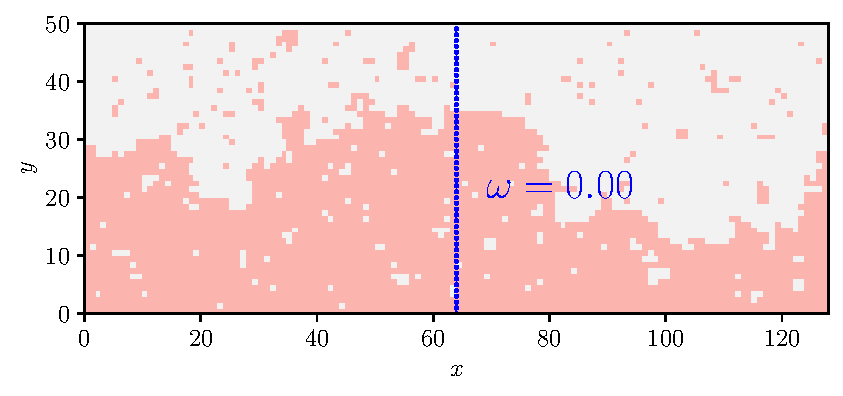
\includegraphics[width=\linewidth]{cis-ising-f-000.pdf}
		\end{minipage}%
		\begin{minipage}[t]{0.5\linewidth}
		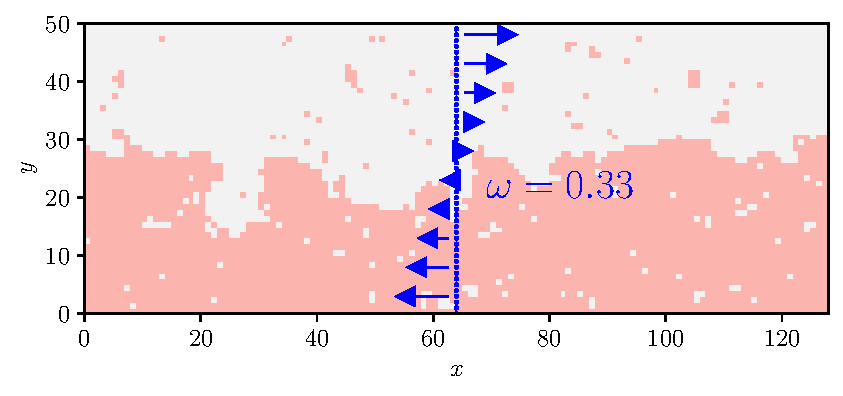
\includegraphics[width=\linewidth]{cis-ising-f-033.pdf}
		\end{minipage}
		\begin{minipage}[c]{0.5\linewidth}
		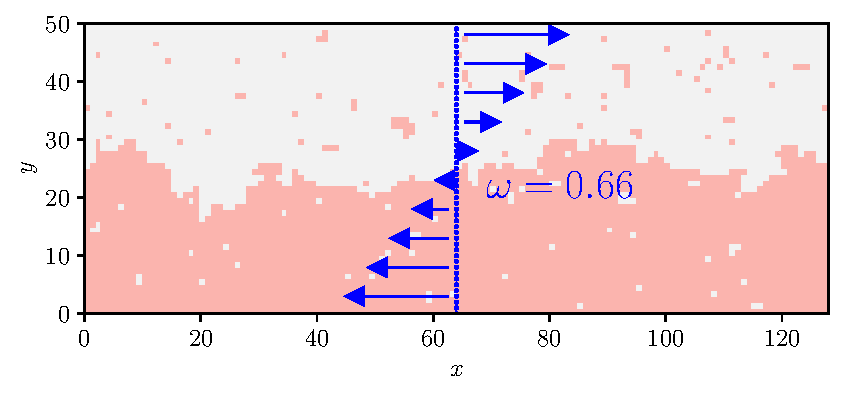
\includegraphics[width=\linewidth]{cis-ising-f-066.pdf} 
		\end{minipage}
    \end{figure}  
    \centering
	Snapshots of 2D Ising driven systems for $T=0.9 T_C$
	\onslide<2>
	\begin{columns}
	\column{0.45\linewidth}
		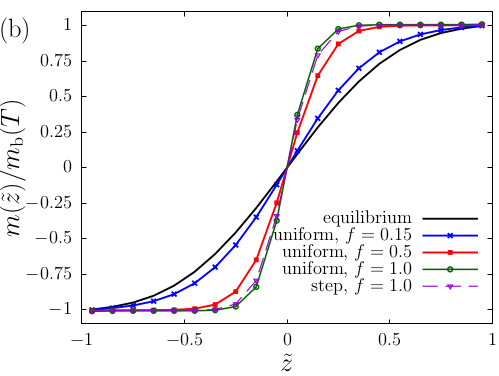
\includegraphics[width=\linewidth]{smith-mag.png} \\
		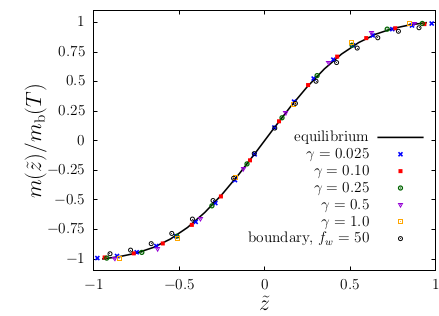
\includegraphics[width=\linewidth]{smith-rescale.png}
	\column{0.45\linewidth}
		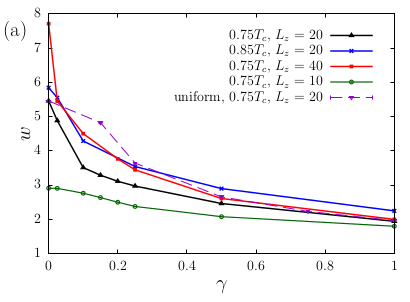
\includegraphics[width=0.9\linewidth]{smith-width.png}
	    Magnetisation profiles, rescaled magnetisation profiles, interfacial width with respect to shear for different $L_Y$
	\end{columns}
    \end{overprint}       
\end{frame}


\begin{frame}
    \frametitle{Binary mixture under laser radiation pressure [Delville et al. 08 (J. Opt. A)]}
    \centering
    \begin{figure}
    	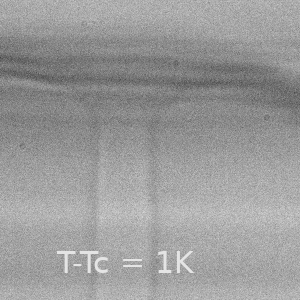
\includegraphics[width=0.3\linewidth]{raph-1k.png}
    	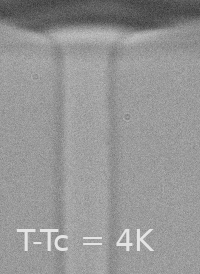
\includegraphics[width=0.3\linewidth]{raph-4k.png}
    	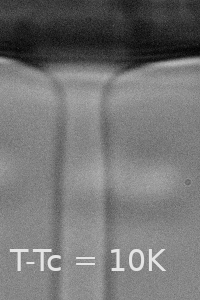
\includegraphics[width=0.3\linewidth]{raph-10k.png}    	    	
    \end{figure}
    {\small Quaternary liquid mixture made of toluene, sodium dodecyl sulfate (SDS), n-butanol and water gives 2 separate micellar phases } \\
\end{frame}

\begin{frame}
    \frametitle{Imposed hydrodynamic flow}
    Advecting the field $\psi(\bx,t)$ with a flow $\bv(\bx)$ gives
    \begin{equation}
       \frac{\partial \psi(\bx,t)}{\partial t} + \nabla \cdot ( \bv \psi(\bx,t) ) = D\nabla^2\frac{\delta H}{\delta \psi(\bx)}+ \sqrt{2D T}\nabla \cdot {\bm \eta}_1(\bx,t) 
    \end{equation}

    \centering
    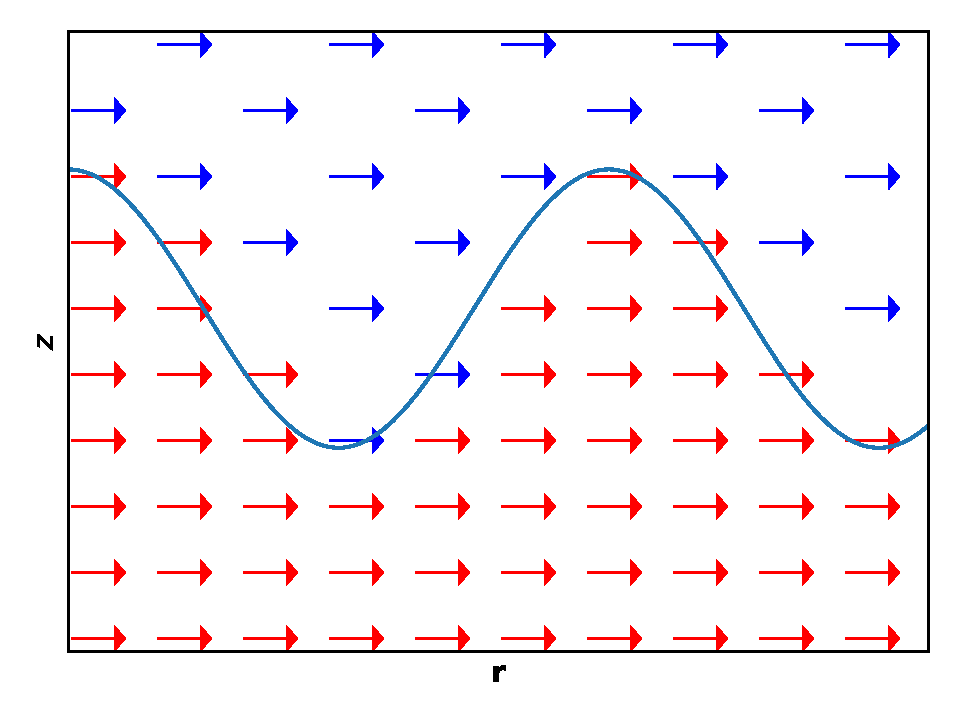
\includegraphics[scale=0.4]{driven.pdf}  \\
    Uniform advecting flow $\bv(\bx,t) = v {\bf e}_x$ in the {\bf sharp interface approximation}, galilean invariance $\bx \to \bx + v t$
\end{frame}

\begin{frame}
    \frametitle{The effect of driving on model C interfaces [Dean, Gersberg,Holdsworth 2020 (17)]}
    $\textcolor{blue}{\psi}$ : colloid field under model B dynamics \\
    $\textcolor{OliveGreen}{\phi}$ : passive solvent under model A dynamics \\    

    \begin{align}
        H[\textcolor{blue}{\psi},\textcolor{OliveGreen}{\phi}] =& H_1[\textcolor{blue}{\psi}] +H_2[\textcolor{blue}{\psi},\textcolor{OliveGreen}{\phi}] \\
        H_1[\textcolor{blue}{\psi}]  =&  \int d\bx\left[\frac{\textcolor{Maroon}{\kappa}}{2}[\nabla\textcolor{blue}{\psi}(\bx)]^2 + \textcolor{magenta}{V}(\textcolor{blue}{\psi}(\bx)) - \textcolor{BurntOrange}{g}z \textcolor{blue}{\psi}(\bx)\right] \\
        H_2[\textcolor{blue}{\psi},\textcolor{OliveGreen}{\phi}] =&\int d\bx \frac{\textcolor{Bittersweet}{\lambda}}{2}(1-\textcolor{blue}{\psi}(\bx)-\textcolor{OliveGreen}{\phi}(\bx))^2
    \end{align}

    $\textcolor{Maroon}{\kappa}$ : interface energy \\
    $\textcolor{magenta}{V}$ : phase separating potential \\
    $\textcolor{BurntOrange}{g}$ : gravitational term introducing finite size correlations \\
    $\textcolor{Bittersweet}{\lambda}$ : coupling parameter

\end{frame}
  
\begin{frame}
    \frametitle{Model C dynamics}
    Equations 
	\begin{eqnarray}
	\frac{\partial \textcolor{blue}{\psi}(\bx,t)}{\partial t} +\textcolor{Red}{\bf v}\cdot { \nabla}\textcolor{blue}{\psi}(\bx,t)&=& D\nabla^2\frac{\delta H}{\delta \textcolor{blue}{\psi}(\bx)}+ \sqrt{2D T}\nabla \cdot {\bm \eta}_1(\bx,t) \\
	\frac{\partial \textcolor{OliveGreen}{\phi}(\bx,t)}{\partial t} &=& -\alpha\frac{\delta H}{\delta \textcolor{OliveGreen}{\phi}(\bx)}+ \sqrt{2\alpha T}{ \eta}_2(\bx,t)
	\end{eqnarray}
	are coupled by $H_2$, with a closed form on  $\textcolor{blue}{\psi}$
	
	\begin{align}
	   \underbrace{\frac{\partial \textcolor{blue}{\psi}(\bx,t)}{\partial t}}_{\text{evolution}} -
	    \underbrace{\textcolor{Bittersweet}{\lambda} D\nabla^2\int_{-\infty}^t dt'
	\exp(-\alpha\textcolor{Bittersweet}{\lambda}(t-t')) \frac{\partial \textcolor{blue}{\psi}(\bx,t')}{\partial t}}_{\text{coupling term}}
	+ \underbrace{\textcolor{Red}{\bf v}\cdot\nabla\textcolor{blue}{\psi}(\bx, t)}_{\text{advection}} =  \nn
	\underbrace{D\nabla^2  \mu(\bx,t')}_{\text{model B}} +  \underbrace{\zeta(\bx,t)}_{\text{thermal noise}} 
	\end{align}	
	where 
	\begin{equation}
	    \mu(\bx,t)=\frac{\delta H_1}{\delta \textcolor{blue}{\psi}(\bx,t)}
	\end{equation}
	and 
	\begin{equation}
	    \tilde \zeta(\bx,\omega) = \frac{\sqrt{2\alpha T}D\textcolor{Bittersweet}{\lambda}}{i\omega + \alpha\textcolor{Bittersweet}{\lambda}}\nabla^2\tilde \eta_2(\bx,\omega) +
	\sqrt{2DT}\nabla\cdot\tilde {\bm \eta}_1(\bx,\omega).
	\end{equation}
\end{frame} 
 
\begin{frame}
    \frametitle{Model C interface dynamics}
	    Interface approximation $\textcolor{blue}{\psi}(\bx,t)=f(z-h(\br,t))$ using method of Bray et al. 2001 (9,29)] at first order in $h$
	\begin{align}
	    \textcolor{BlueViolet}{\Delta \psi}^2 \int d{\bf r} G(0,{\bf r}-{\bf r}') [\frac{\partial h({\bf r},t)}{\partial t}    
	    +\textcolor{Red}{\bf v}\cdot\nabla h({\bf r},t)] & =  \textcolor{VioletRed}{\sigma}[\nabla^2 h({\bf r},t) -\textcolor{BurntOrange}{m}^2 h({\bf r},t)] + \xi({\bf r},t) \nn
	    +\frac{\textcolor{VioletRed}{\sigma}\textcolor{Bittersweet}{\lambda} D}{\textcolor{Maroon}{\kappa}}\int_{-\infty}^t dt' 	\exp(-\alpha\textcolor{Bittersweet}{\lambda}(t-t'))\frac{\partial h({\bf r},t')}{\partial t'} & & 
	\end{align}
    where $G= -\nabla^{-2}$,  $\xi({\bf r},t) = \int_{-\infty}^{\infty} dz f'(z-h({\bf r},t)) \nabla^{-2} \zeta(\bx,t)$, $\textcolor{BurntOrange}{m}^2 = \textcolor{BlueViolet}{\Delta \psi} \textcolor{BurntOrange}{g} / \textcolor{VioletRed}{\sigma}$
\end{frame} 
  
 
\begin{frame}
    \frametitle{Model C interface correlation function}
    \begin{block}{Correlation function}
    \footnotesize
		    \begin{align}
		\tilde C_s({\bf q}) = T \frac{\left(2 D\textcolor{VioletRed}{\sigma} q(\textcolor{Maroon}{\kappa}[q^2+\textcolor{BurntOrange}{m}^2]+\textcolor{Bittersweet}{\lambda})+\alpha\textcolor{Maroon}{\kappa}\textcolor{Bittersweet}{\lambda}\textcolor{BlueViolet}{\Delta \psi}^2\right)^2 +\textcolor{Maroon}{\kappa}^2 \textcolor{BlueViolet}{\Delta \psi}^4 ({\bf q}\cdot\textcolor{Red}{\bf v})^2}{\textcolor{VioletRed}{\sigma}[q^2+\textcolor{BurntOrange}{m}^2]\left(2D q\textcolor{VioletRed}{\sigma} (\textcolor{Maroon}{\kappa}[q^2+\textcolor{BurntOrange}{m}^2]+\textcolor{Bittersweet}{\lambda})+\alpha \textcolor{Maroon}{\kappa}\textcolor{Bittersweet}{\lambda} \textcolor{BlueViolet}{\Delta \psi}^2\right)^2 + \textcolor{Maroon}{\kappa}\left(\textcolor{Maroon}{\kappa}\textcolor{VioletRed}{\sigma}[q^2+\textcolor{BurntOrange}{m}^2] + \textcolor{Bittersweet}{\lambda}\textcolor{VioletRed}{\sigma}\right)\textcolor{BlueViolet}{\Delta \psi}^4({\bf q}\cdot\textcolor{Red}{\bf v})^2}
		\end{align}    
    \end{block}


    \begin{columns}
    \column{0.45\linewidth}
        \centering
        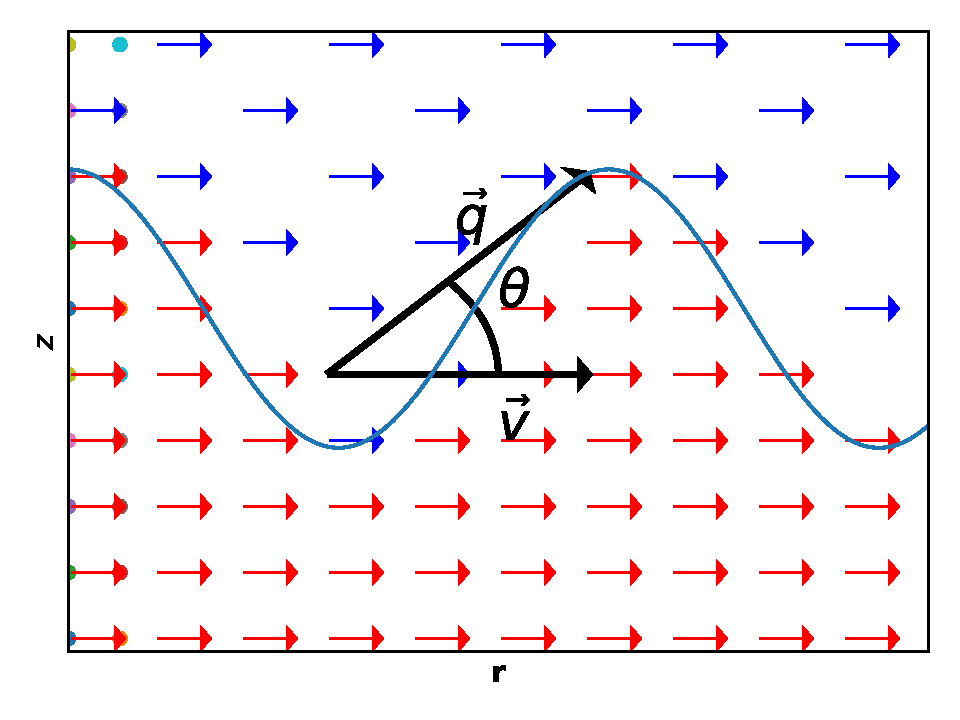
\includegraphics[width=\linewidth]{shear-c.pdf}
    \column{0.45\linewidth}   
    
	\begin{overprint}
	\onslide<1>
	\begin{block}{No driving $v \to 0$}
			    \begin{align}
		\tilde C_s({\bf q}) =  \frac{T}{\textcolor{VioletRed}{\sigma}[q^2+\textcolor{BurntOrange}{m}^2]}
		\end{align} 
	\end{block}
	\begin{block}{Infinite driving $v \to \infty$}
	\begin{align}
		\tilde C_s({\bf q}) =  \frac{T}{\textcolor{VioletRed}{\sigma}[q^2+\textcolor{BurntOrange}{m}^2+\frac{\textcolor{Bittersweet}{\lambda}}{\textcolor{Maroon}{\kappa}}]}
	\end{align}
	\end{block}
	\onslide<2>
	\vspace{-0.5cm}
	\begin{block}{Small $\bq$ approximation}
		\begin{itemize}
		\item  Angle-dependent surface tension
		\begin{equation}
		    \textcolor{VioletRed}{\sigma_s}(\theta) = \textcolor{VioletRed}{\sigma}(1+ \frac{\textcolor{red}{v}^2\cos^2(\theta)}{\textcolor{red}{v_0}^2})
		\end{equation}
		\item Angle-depentent correlation length
		\begin{equation}
		    \xi_s = \xi_{eq}\sqrt{1+ \frac{\textcolor{red}{v}^2\cos^2(\theta)}{\textcolor{red}{v_0}^2}}
		\end{equation}
		\item Intrinsic velocity 
		\begin{align}
		\textcolor{red}{v_0} = \sqrt{\alpha^2\textcolor{Bittersweet}{\lambda}\textcolor{Maroon}{\kappa}}
		\end{align}
		\end{itemize}
	\end{block}
	\end{overprint}		
	\end{columns}

\end{frame} 

\section{Conclusion}

\begin{frame}
    \frametitle{Presentation's conclusion}
    \begin{block}{Driven Solid-On-Solid model}
    \begin{itemize}
    	\item Explanation of the model 
        \item Driven does increase interface width, as in wind generated waves
    \end{itemize}
    \end{block}    
    \begin{block}{Driven Model C}
    \begin{itemize}
    	\item Similarities between shearing and driving
    	\item Steady-state out-of-equilibrium driving needs a coupling between two fields due to Galilean invariance (model C)
        \item Increase of the effective surface tension in the direction of driving and also an increase in the correlation length of the height fluctuations with respect to a non-driven equilibrium interface
        \item Uniform driving leads to effective equilibrium statistics
    \end{itemize}
    \end{block}
\end{frame} 

\begin{frame}
	\frametitle{Thesis' conclusion}
	\begin{block}{Chapter 3 : Equilibrium Interface models and their finite size effects}
	\begin{itemize}
		\item General method to compute free energy and probability distribution functions of continuous gaussian interfaces with path integral method
		\item Generalization the Lopes Cardozo-Jacquin-Holdsworth method to compute free energy in numerical Monte Carlo lattice systems for any type of external potentials, useful for Kawasaki dynamics
		\item Exact diagonalization of the finite Solid-On-Solid transfer matrix
	\end{itemize}
	\end{block}
	\begin{block}{Chapter 4 : Beyond Solid-On-Solid : the Particles-Over-Particles model}
	\begin{itemize}
		\item New model generated from SOS with entropic term
		\item Multi-particles formulation 
		\item Numerical Monte Carlo issues : corner case of Metropolis algorithm
		\item Actually is the model that gaves us the computational idea for model C (the paper)
	\end{itemize}
	\end{block}	
	\begin{block}{Chapter 5 : Driven interfaces}
	\begin{itemize}
		\item Presentation's conclusion
	\end{itemize}	
	\end{block}
\end{frame}

\begin{frame}
	\frametitle{Overall conclusion}
	\begin{itemize}
		\item Relationship between continuous gaussian and discrete solid-on-solid models (Eq. 3.84 and 3.184), with surface tension computations
		\item Casimir-type effect have an interesting manifestation in interface physics, 
		\item Interface models have no bulk free energy, only excess free energy due to confinement 
		\item Casimir-like effect is seen in interface models in the critical regime $\sigma \to 0$
		\item POP systems allow for particles coupling with different temperatures or thermodynamical ensembles (model C) and different hydrodynamical flows
		\item SFT explanation as to why driving increases surface tension and correlation length along the interface
		\item Driven steady-states do have equilibrium properties
	\end{itemize}
\end{frame}

\begin{frame}
    \frametitle{Perspectives}
    \begin{itemize}
    	\item Thanks to the generalized free energy computation method, study the difference between thermodynamical ensembles on finite-size critical systems
    	\item Get deeper on the relationship between critical and interface systems
    	\item Solve POP's numerical problems. Study coupled systems as presented model C through it
    	\item Better understand the difference between driving at interface and bulk driving
    	\item Do out-of-equilibrium confined interfaces have different physics than equilibrium confined ones ?
    \end{itemize}
\end{frame}


\end{document}


 
 